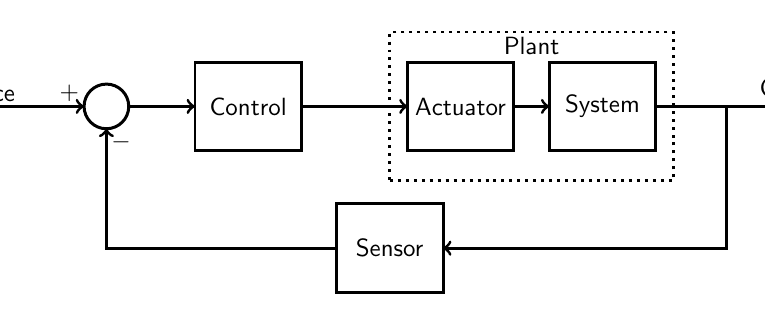
\begin{tikzpicture}[inner sep=0pt,outer sep=0pt,very thick,
sysblock/.style={draw,rectangle,inner sep=2pt,minimum width=1.5cm,minimum height=1.25cm,very thick}]
\useasboundingbox (-1,1) rectangle (8,-2.5); 
\begin{scope}[transform canvas={scale=.9}]
\draw (0,0) node[draw,circle] (sum) {$\rule{0pt}{18pt}$};
\draw (2,0) node[sysblock] (C) {\textsf{Control}};
\draw (5,0) node[sysblock] (A) {\textsf{Actuator}};
\draw (7,0) node[sysblock] (G) {\textsf{System}};
\draw (6,0) node[draw,rectangle,dotted,minimum width=4cm,minimum height=2.1cm] {};
\draw (6,.85) node {\textsf{Plant}};
\draw (4,-2) node[sysblock] (H) {\textsf{Sensor}};

\draw[->] (-2,0) node[above=2pt] {\textsf{Reference}} -- (sum.180) node[above left=2pt] {$+$};
\draw[->] (sum.0) -- (C);
\draw[->] (C) -- (A);
\draw[->] (A) -- (G);
\draw[->] (G.0) -- ++(2,0) node[above=2pt] {\textsf{Output}};
\draw[->] (G.0) -- ++(1,0) |- (H);
\draw[->] (H) -| (sum.-90) node[below right=2pt] {$-$};
\end{scope}
\end{tikzpicture}
